\section{Testing of the PlayStation Controller} \label{sec:ps_testing}

\subsection{Frequency Response Function}%explain why it is important
For an in-depth performance analysis and evaluation of the controller a series of experiments have been conducted. A standard approach is to measure the frequency response function of the controller.\\
In order to find this frequency response, one should consider the amplitude correlation between the input signal and the output signal, as given in the following equation:
\begin{equation}
	H = \frac{F^*(j\omega)}{F(j\omega)}
\end{equation}
Where $F^*(j\omega)$ is the transfer function of the output signal and $F(j\omega)$ of the input signal.\\
The results of this testing can be plotted in a Bode-plot which is a standard representation. This not only shows for which frequencies the reference signal can be tracked nicely, but it also indicates any eventual oscillation frequencies. In addition, one can read out the order of the system when looking at the phase plot of the frequency response function. In the phase plot the phase lag between the reference signal and the output signal is represented. Furthermore, the bode plots allow for a direct cross-platform comparison with other controllers and devices.

\subsection{Test Setup}
In this experiment a thorough frequency response analysis shall be done on the controller. On the left-hand side the motor with a reduction ratio of $33:1$ has been used, whereas for the right-hand side, the motor had a reduction ratio of $112:1$. \\
A reference signal is fed into the Arduino, which then controls the motors to match the compression of the springs with the reference. The operational distance of the photoreceptors to the palm pads is $2$ to $4$mm which lies within the more sensitive region of the sensor.
	
\subsection{Control Scheme}
The reference signal is given by the Function Generator \textbf{SG-4115}. This generator has an intrinsic output impedance of $50$Ohm. This means, that it expects to have a device connected to it with the same value as input impedance. If this is the case, these two elements form a simple voltage divider and only half of the voltage is applied to the target device. However, this is not the case for the Arduino, since it has a considerably higher input impedance. Therefore, the settings made on the function generator result in double the voltage on the Arduino. From this point on, this issue shall be neglected and all future voltage indications refer to the voltage level as seen by the Arduino.\\
The function generator produces a sine wave between $0$ and $5$V with a frequency ranging from $1$ to $100$Hz. The Arduino reads this voltage and controls the motor to have a proportional spring compression accordingly. In this case $0$V as reference signal is $0\%$ compression and $5$V corresponds to $100\%$ compression. The control scheme of this setup can be seen in figure \ref{fig:frf_measure_points}.
\begin{figure}[h!]
	\centering
	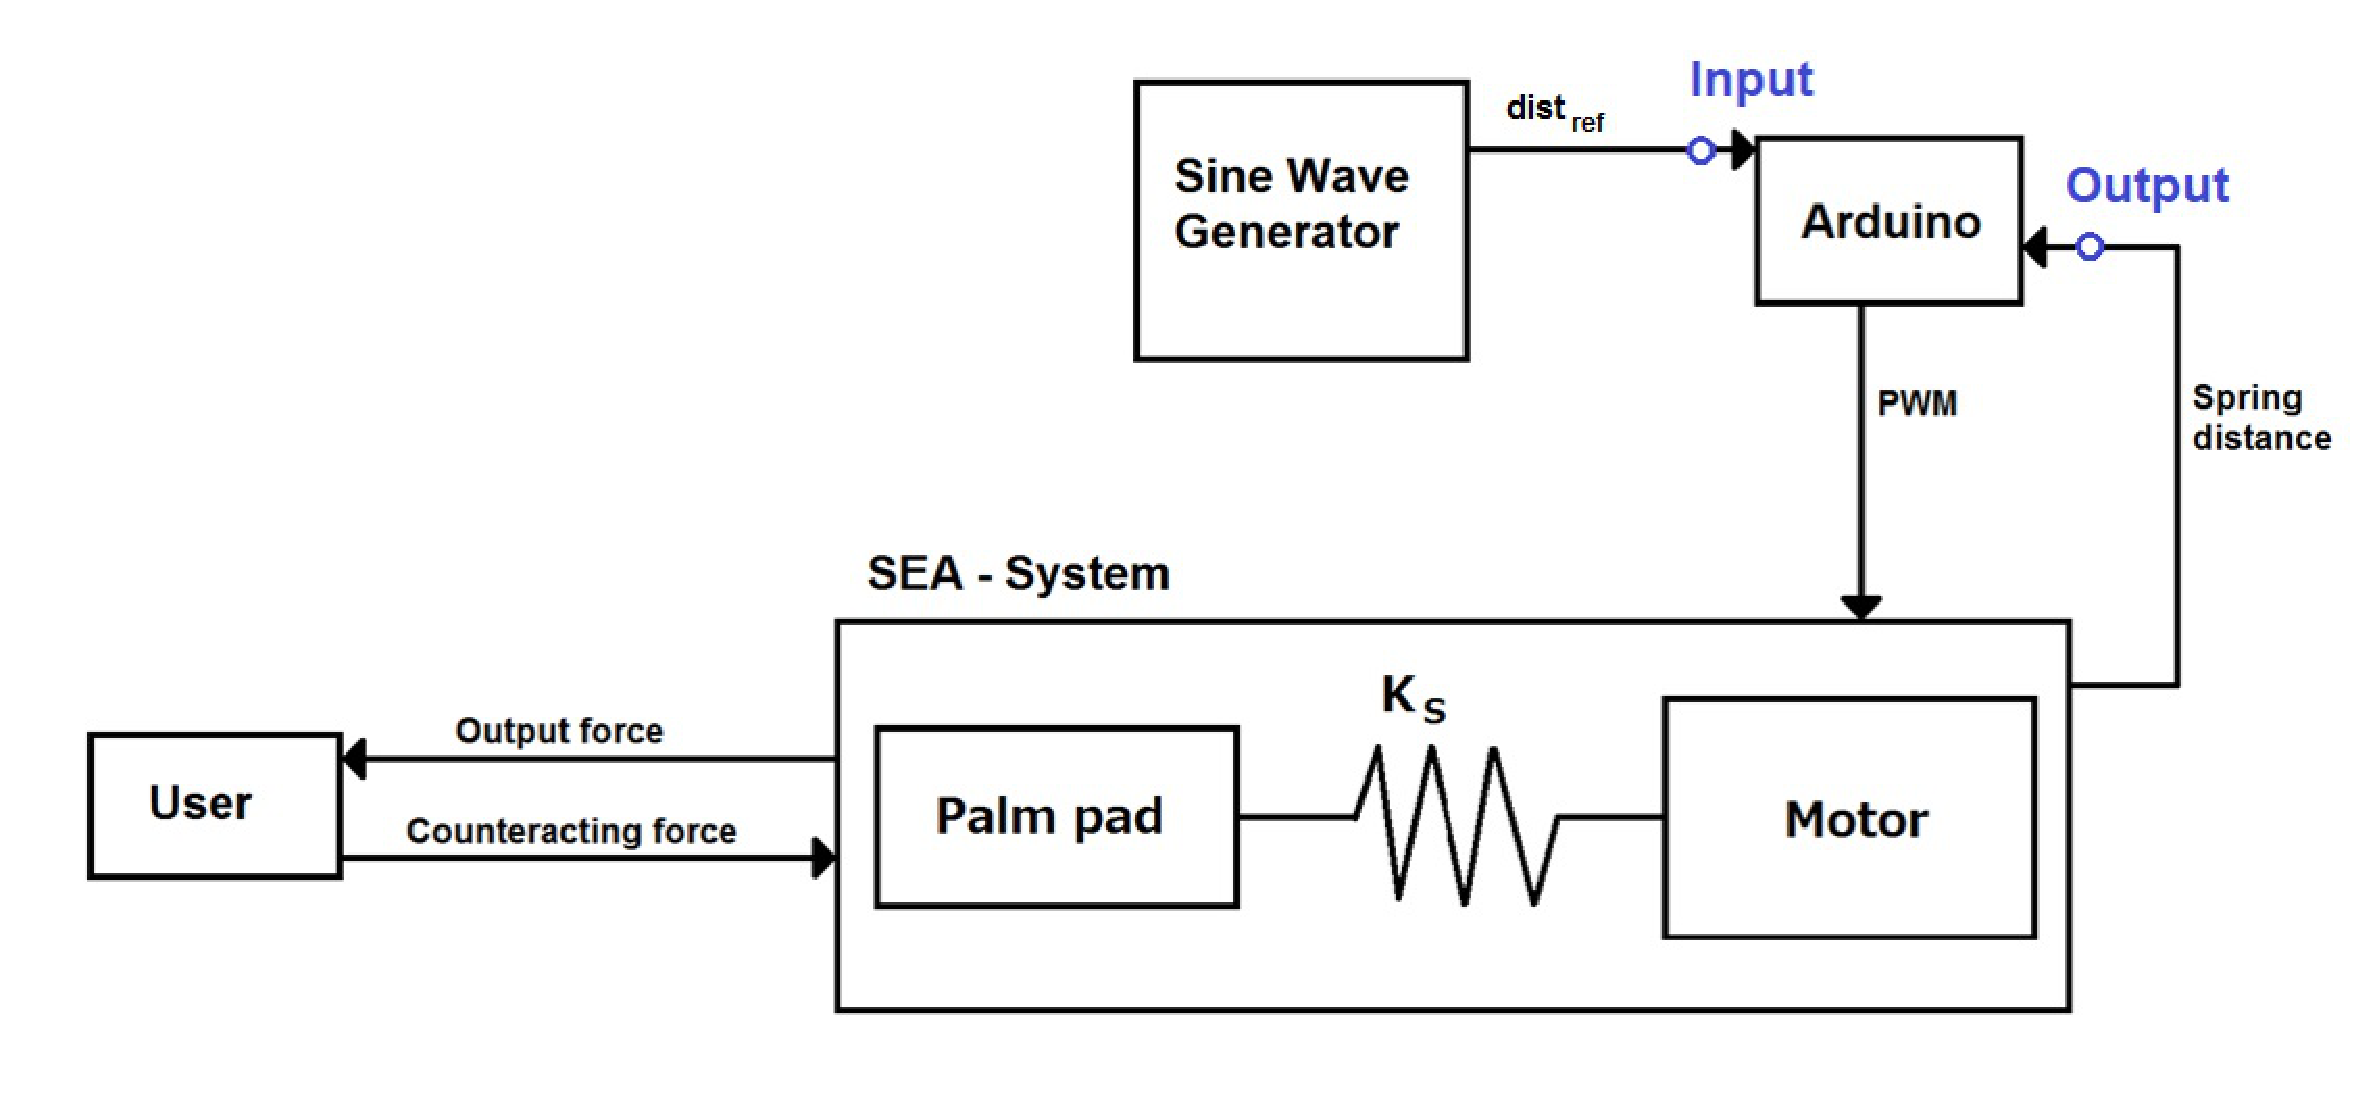
\includegraphics[width=0.6\linewidth]{Figs/frf_measure_points}
	\caption{Control scheme for the frequency response analysis.}
	\label{fig:frf_measure_points}
\end{figure}
In this case the counteracting force from the user is infinite (ie. pseudo-infinite stiffness), since the palm pads have been blocked by a wall. Tests have also been made where the palm pads have been blocked by the operators hands, but without any significant difference. For simplicity, the wall blocked test setup has been used for future investigation.


\subsection{Tracking Behavior of the P-controller}
In order to measure the tracking performance of the controller, the Arduino sent its data to the serial link. This data has then been read and treated in a python script and represented with the \textit{matplotlib} library. \\
The tracking behavior of the P-controlled ($K_P = 39.2$V/mm) setup can be seen in the following figures.

\begin{figure}[h!]
    \centering
    \begin{minipage}{0.45\textwidth}
        \begin{figure}[H]
        	\centering
        	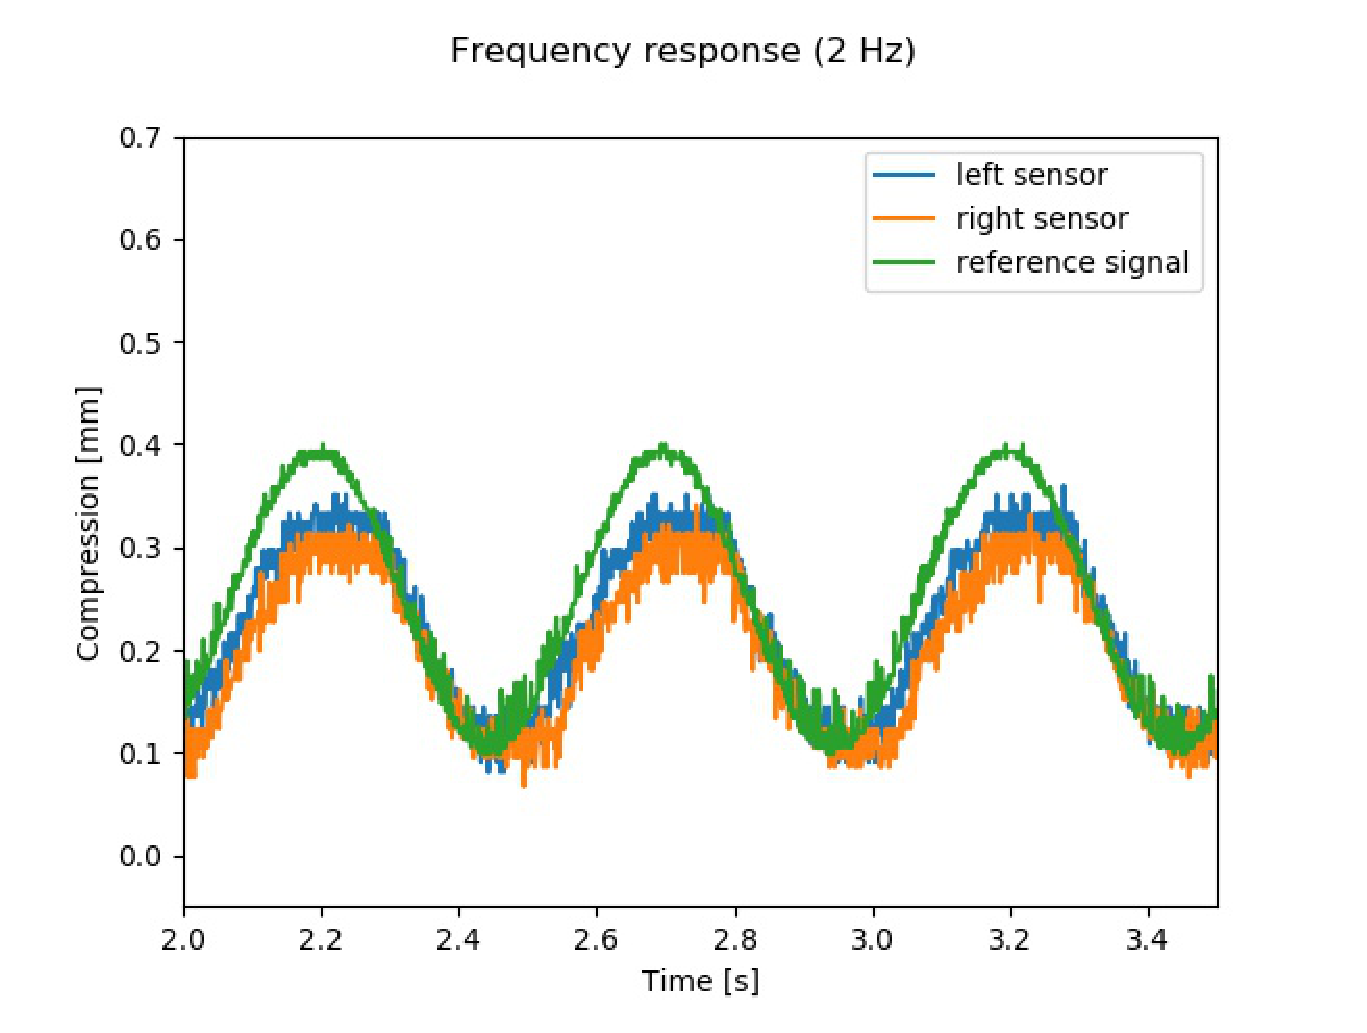
\includegraphics[width=1.0\linewidth]{Figs/2plot_zoom_P}
        	\caption{Tracking behavior of the P-controller ($K_P = 39.2$V/mm) for $2$ Hz.}
        	\label{fig:2plot_zoom_P}
        \end{figure}
    \end{minipage}
    \begin{minipage}{0.45\textwidth}
        \begin{figure}[H]
        	\centering
        	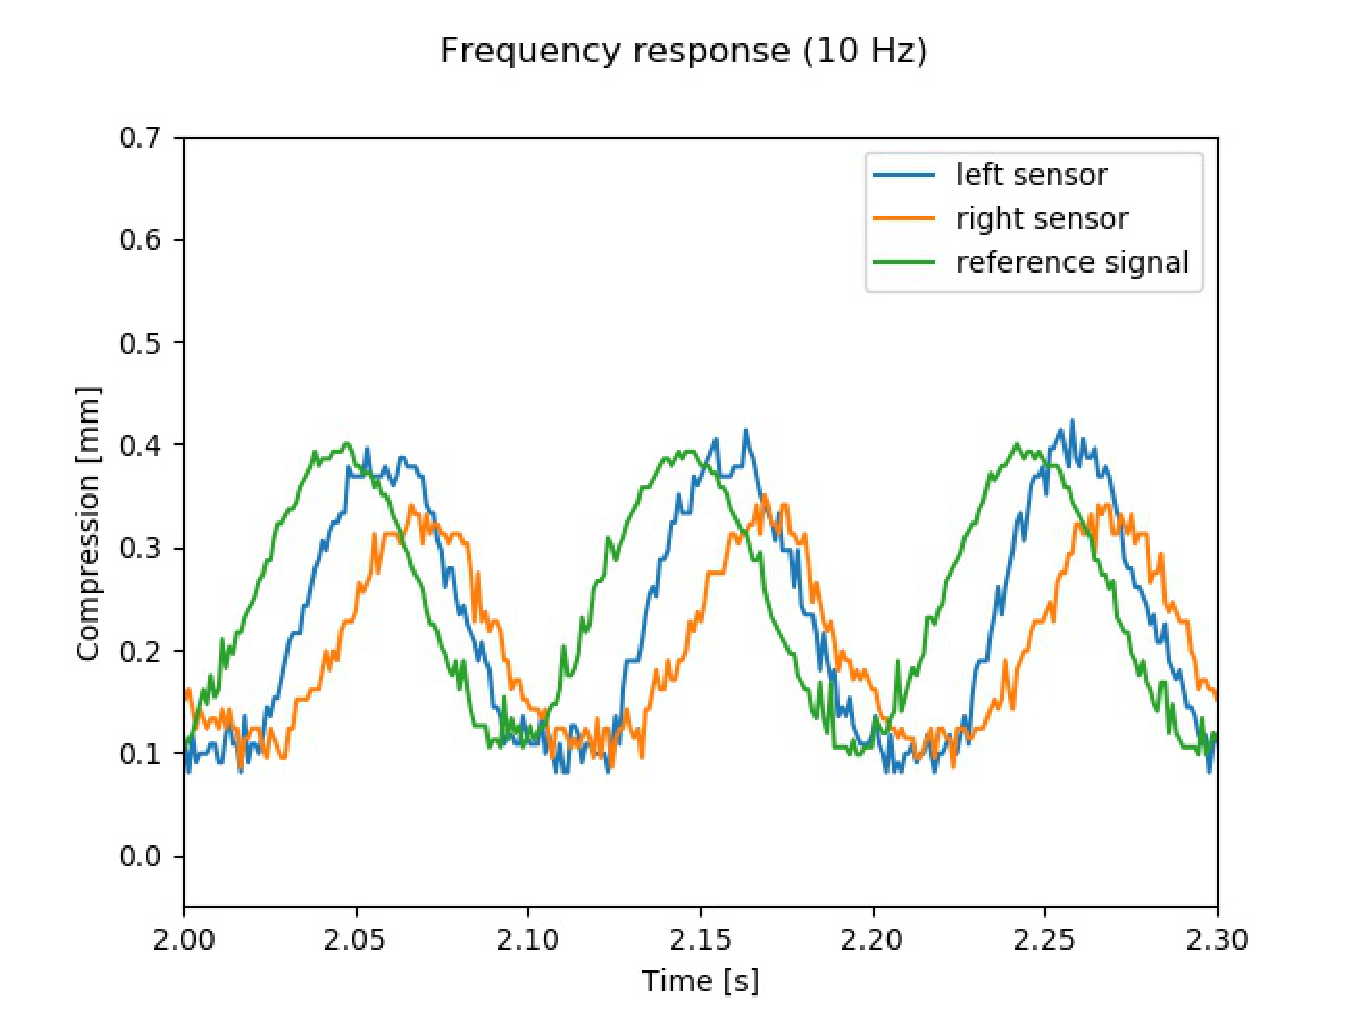
\includegraphics[width=1.0\linewidth]{Figs/10plot_zoom_P}
        	\caption{Tracking behavior of the P-controller ($K_P = 39.2$V/mm) for $10$ Hz.}
            \label{fig:10plot_zoom_P}
        \end{figure}
    \end{minipage}

\end{figure}


\subsection{Sinewave Fitting}
As described in this example\cite{exnumerus2010}, one can fit a sinewave with the linear least square method to the samples. For finding the amplitude the second norm has been used. This function returns the phase, amplitude and the bias. In this case, the difference in phase between input and output, as well as the amplitude ratio is needed in order to plot a Bode diagram.


\subsection{Experimental PID Tuning}
At first, the Ziegler Nichols tuning method has been used to identify the PID gains for the setup. However, due to the non-linear behaviour, these gains resulted in a rather poor tracking performance of the reference signal.\\
Since an educated tuning of the gains is the very core problem of all control engineering, a lot of different approaches exist to find optimal or sub-optimal gain values. Given the complexity of the setup, it seemed reasonable to go for the simple trial and error approach, where the gains have been tuned and the tracking performance was shown in real-time. This approach led to the following gain coefficients:

\todo[inline]{discuss the fact of neglected efficiency, what is backdriveability exactly, redo bode plot with new pid settings }
\begin{figure}[h!]
	\centering
	\begin{tabular}{|l|c|c|}
		\hline
		Designator & Value & Unit \\ \hline \hline
		$K'_P$ & $47.6$ & [V/mm]\\ 
		$K'_I$ & $0.124$ & [V/mm/s]\\
		$K'_D$ & $247$ & [Vs/mm]\\
		\hline
	\end{tabular}
	\caption{Trial and error PID tuning.}
	\label{tab:trial_error_pid}
\end{figure}


\subsection{Tracking Behavior of the PID-controller}
The tracking behavior of the PID-controlled setup can be seen in the following figures.



\begin{figure}[h!]
    \centering
    \begin{minipage}{0.45\textwidth}
        \begin{figure}[H]
        	\centering
        	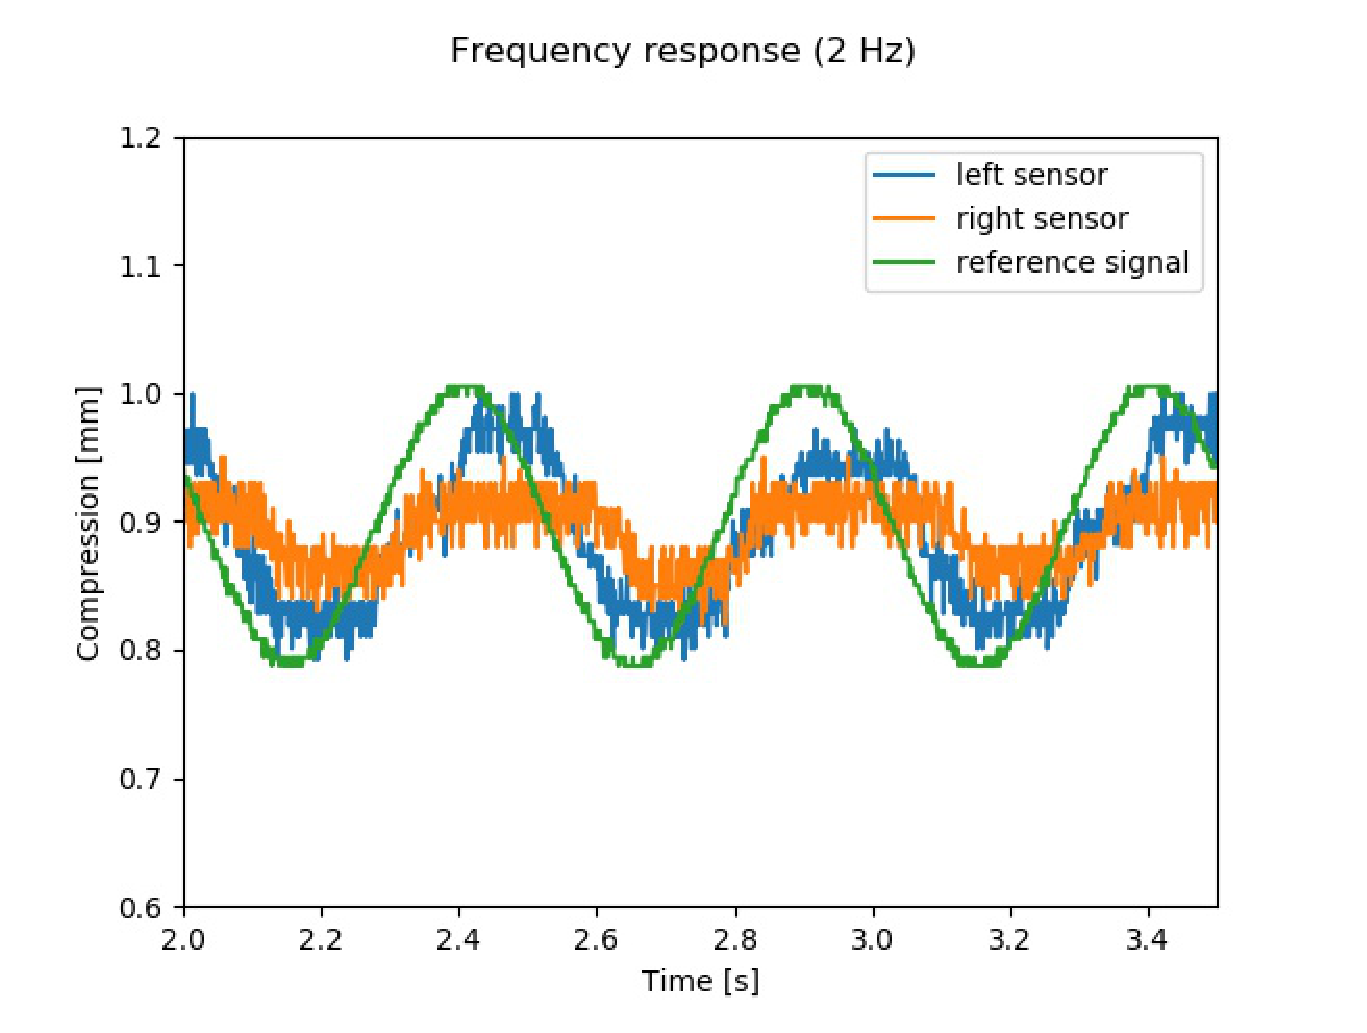
\includegraphics[width=0.6\linewidth]{Figs/2plot_zoom_PID}
        	\caption{Tracking behavior of the PID-controller (see table \ref{tab:trial_error_pid}) for $2$ Hz.}
        	\label{fig:2plot_zoom_PID}
        \end{figure}
    \end{minipage}
    \begin{minipage}{0.45\textwidth}
        \begin{figure}[H]
        	\centering
        	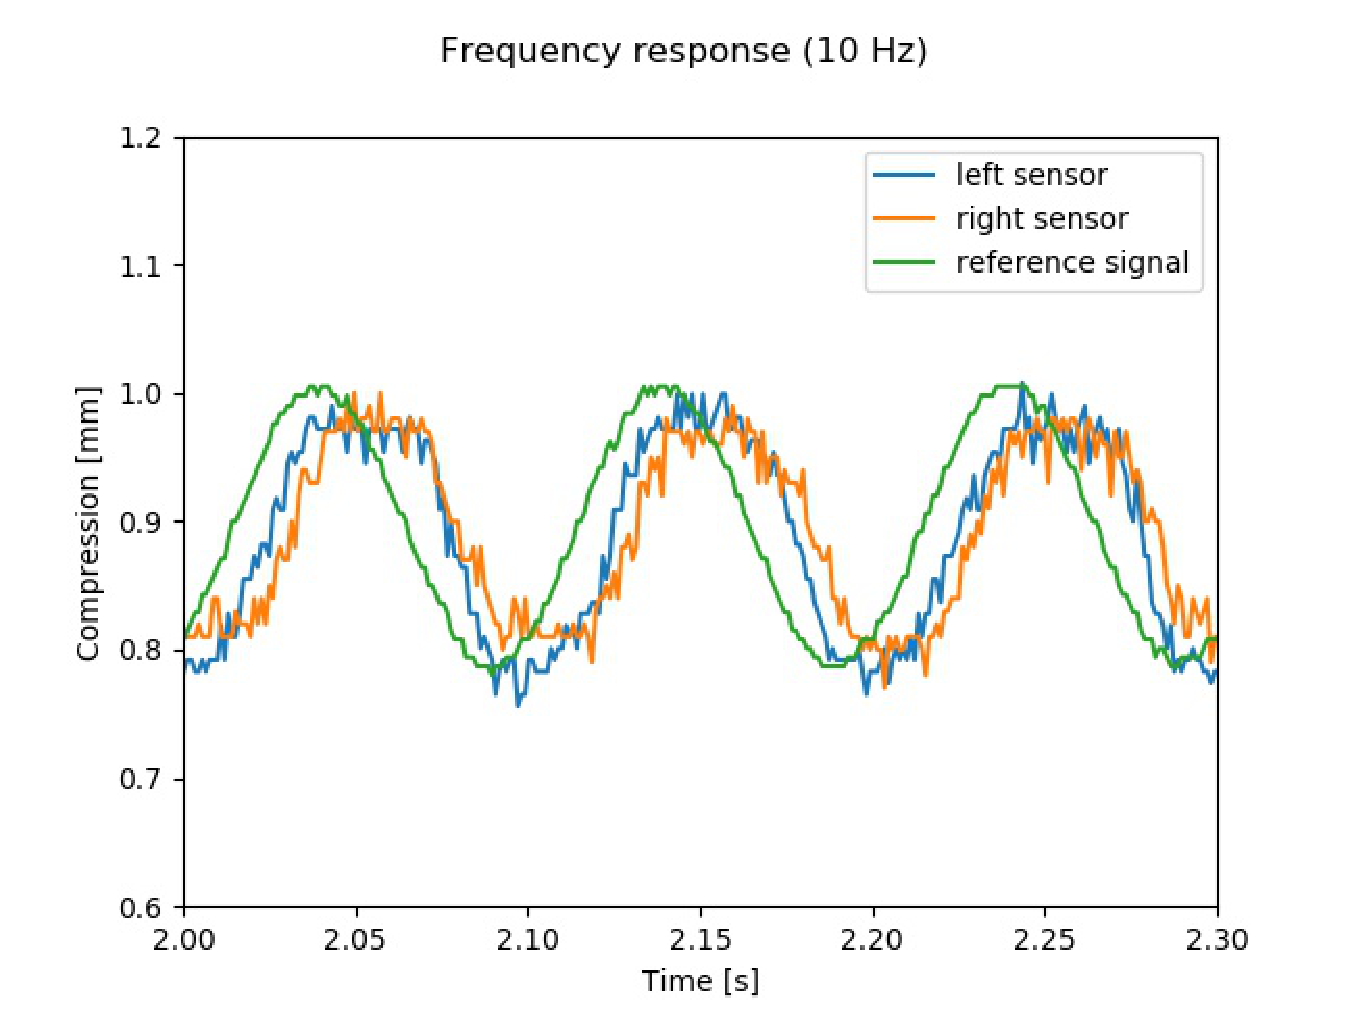
\includegraphics[width=0.6\linewidth]{Figs/10plot_zoom_PID}
        	\caption{Tracking behavior of the PID-controller (see table \ref{tab:trial_error_pid}) for $10$ Hz.}
        	\label{fig:10plot_zoom_PID}
        \end{figure}
    \end{minipage}
\end{figure}


\subsection{Performance Evaluation}
\begin{figure}[h!]
	\centering
	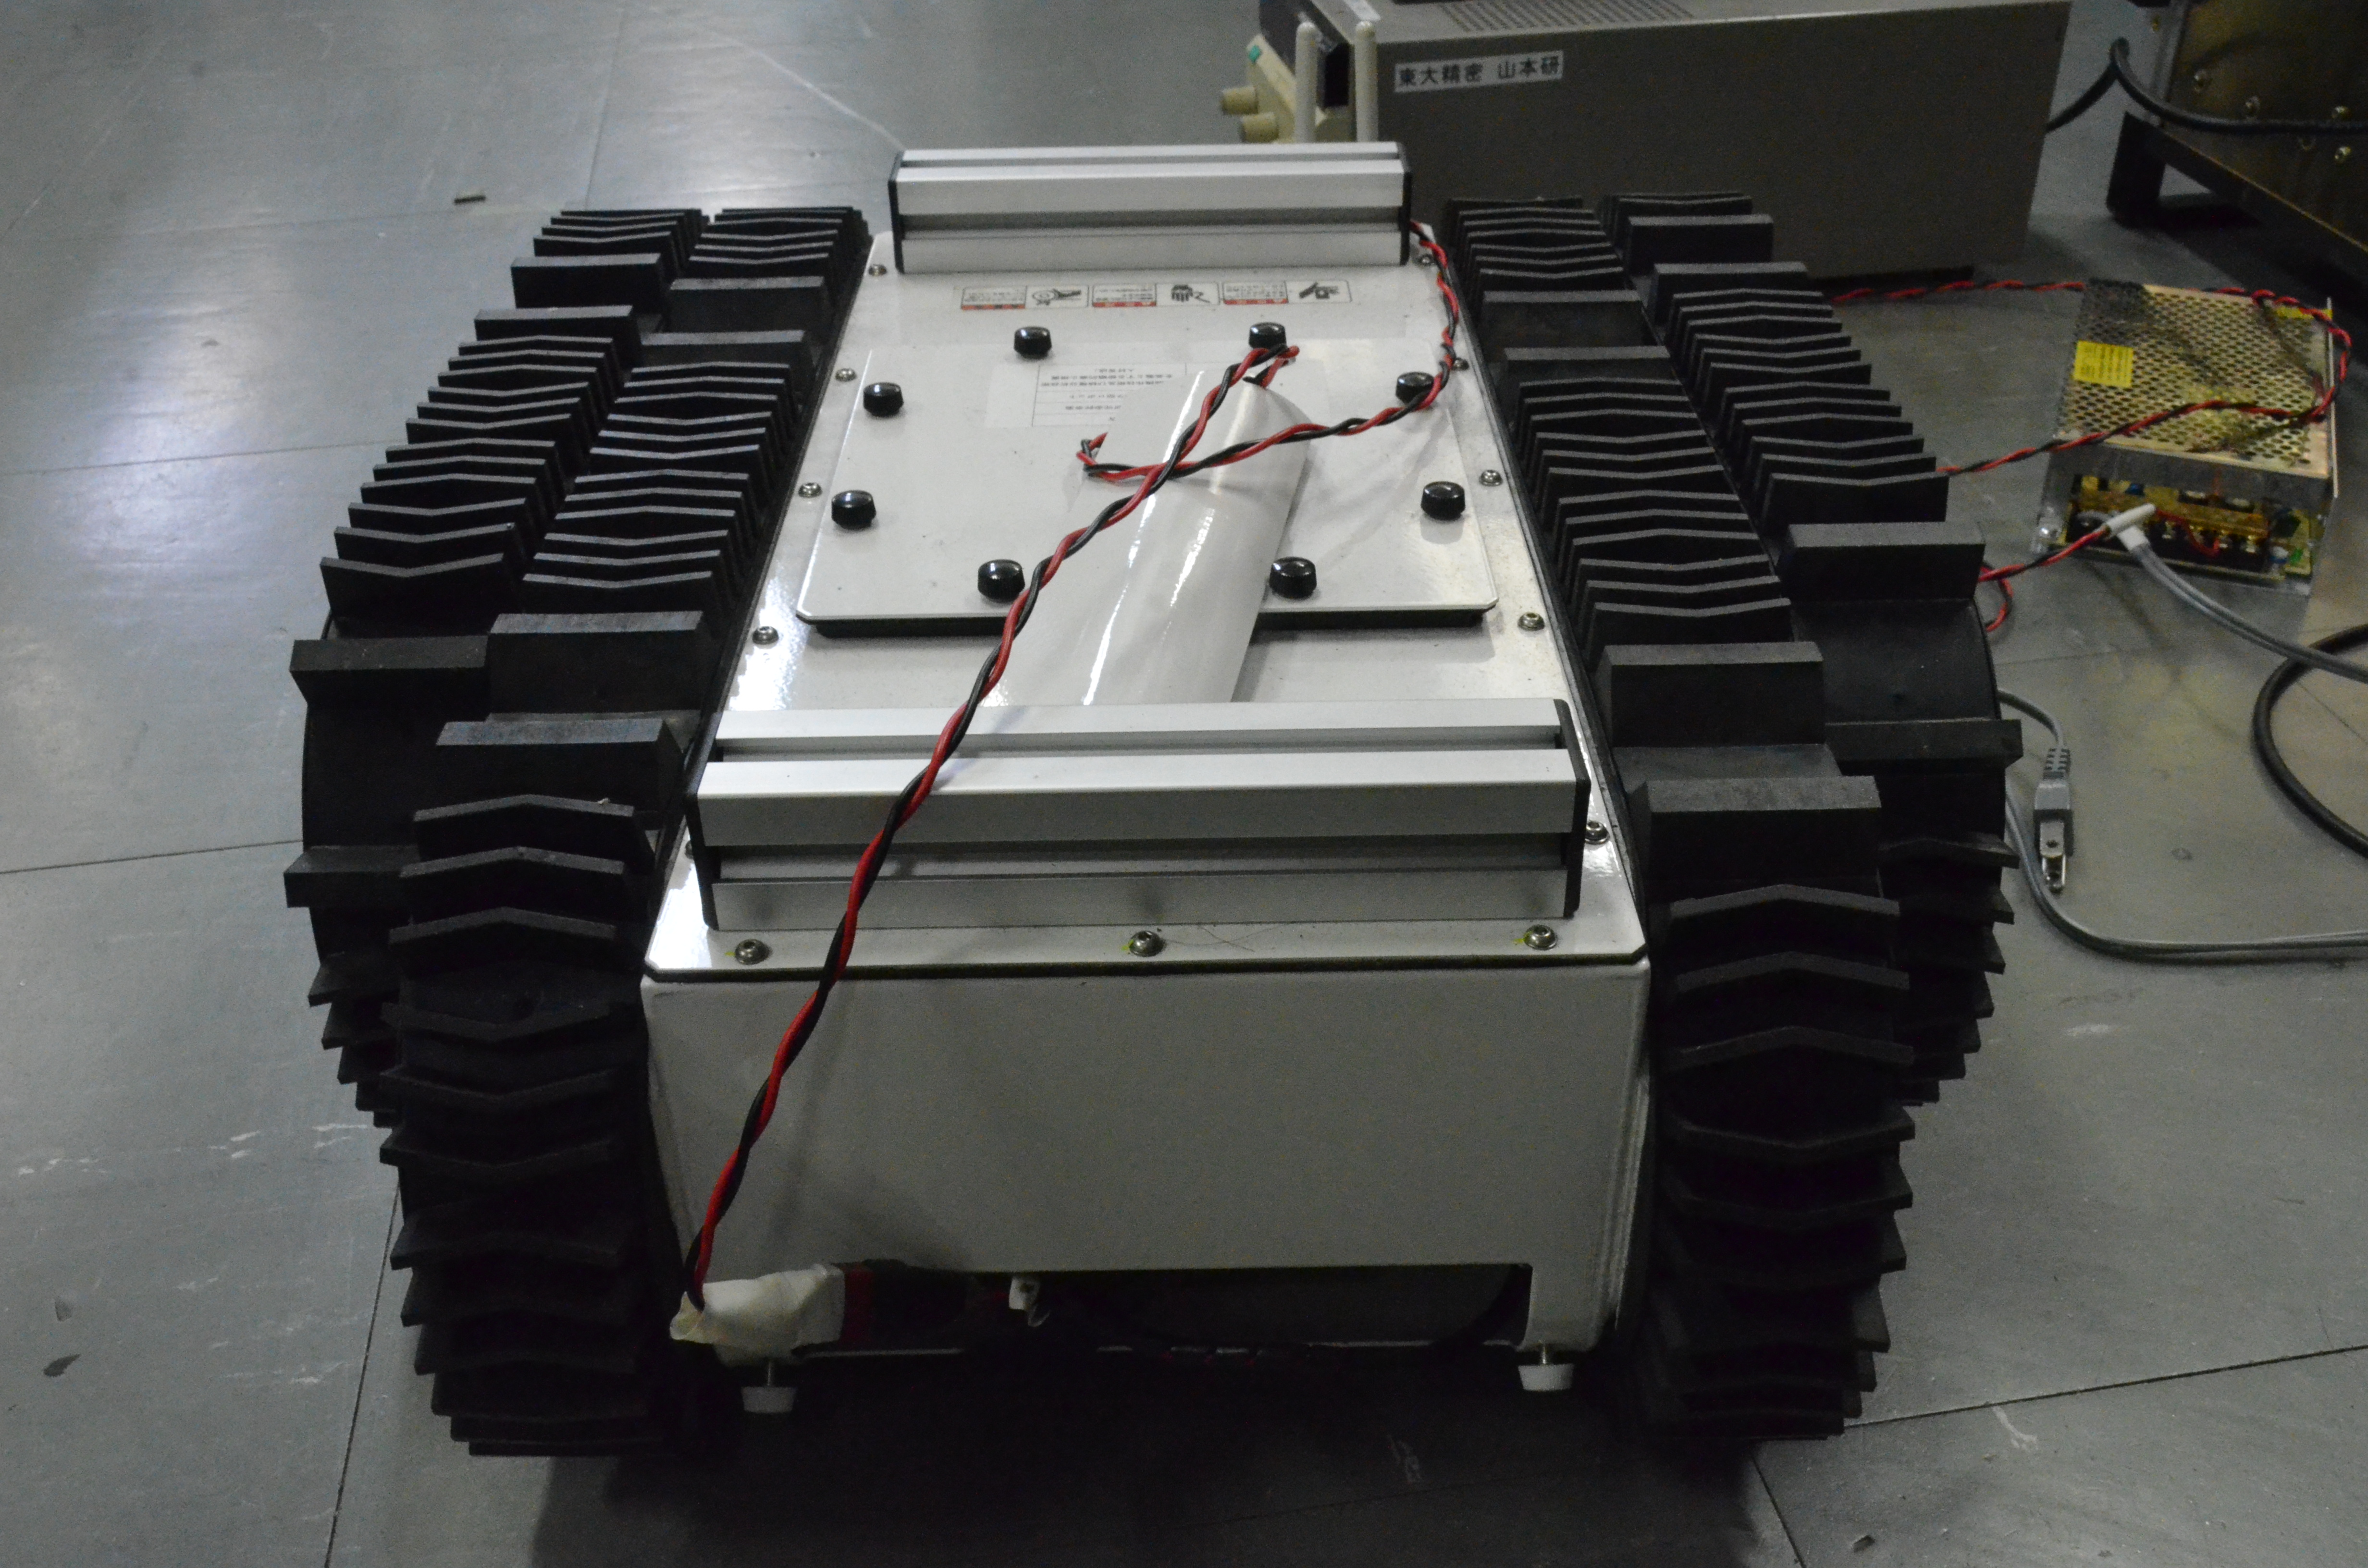
\includegraphics[width=0.6\linewidth]{Figs/topy_robot}
	\caption{Topy robot for real-world controller test setup.}
	\label{fig:topy_robot}
\end{figure}
After having found gains that seem to work well enough for the desired application, the PlayStation-controller setup has been put to the test. At first, the controller has been connected to the computer to communicate with the Topy robot. 

\subsubsection{Latency}
The controller was successfully able to navigate the robot, if with a delay of roughly $700$ms. The commercial controller, that was developed for the Topy robot, also had a certain delay of almost $500$ms. This delay is the difference between the instant when the joystick is pushed forward, and the moment when the robot starts moving. The feedback methods that have been tested varied between a pure pitch feedback, a combined pitch and roll feedback and a current consumption feedback law. \todo[inline]{state feedback laws and reference here}\\
The effect and magnitude of the command latency, but also of the feedback latency can be seen in figure \ref{fig:real_P_scope_13_latency_plot} and \ref{fig:real_PID_scope_14_latency_plot}.

\begin{figure}[h!]
	\centering
	\includegraphics[width=1\linewidth]{Figs/real_P_scope_13_latency_plot}
	\caption{Command and behavior of Topy robot with P-controlled PlayStation controller.}
	\label{fig:real_P_scope_13_latency_plot}
\end{figure}


\begin{figure}[h!]
	\centering
	\includegraphics[width=1\linewidth]{Figs/real_PID_scope_14_latency_plot}
	\caption{Command and behavior of Topy robot with PID-controlled PlayStation controller.}
	\label{fig:real_PID_scope_14_latency_plot}
\end{figure}



In these figures, several interesting things have to be mentioned. First of all, the delay between sending the commands and receiving the consumed current value, which is then used as feedback value, is roughly $700$ms. The delay between the received feedback value and the response of the distance sensor is much smaller and depends on the situation of the robot. When the robot starts to move, it takes some time until the current has built up, and the latency between the reference compression and actual compression is roughly $130$ms for the P-controlled, and $430$ms for the PID-controlled setup (see first red vertical lines). However, when the robot is stopped, the latency is $20$ - $30$ms (second and third red lines).\\
In the first green lines, an external force has been applied to the robot, simulating an obstacle, which increased the consumed current and therefore also increased the desired feedback value. Again, the latency was of roughly $30$ms. The second green lines is where the external force has been removed and the current dropped abruptly back to its normal value. The latency here was below $10$ms.\\
Also indicated in figures \ref{fig:real_P_scope_13_latency_plot} and \ref{fig:real_PID_scope_14_latency_plot}, one can see that the feedback has been turned off when driving backwards (black lines). However, in this scenario the feedback has been activated when standing still, ie. sending $0$ as driving speed. Since the robot is only sending the magnitude but not the direction of the current in the crawlers, the remaining current from the backward motion is fed back. This mode can easily be turned off, such that no feedback is felt when the robot is halting. For reasons of completeness however, this has not been turned off and it is interesting to note, that the time between switching the command values and the reception of the feedback value has been reduced to roughly $50$ms. \\
From these experiments one can conclude that the robot takes a long time to start driving, mainly due to internal implementation of the crawler control scheme. The total delay for this initial start-up is $820$ms for the P-controlled and $1160$ms for the PID-controlled version. The communication delay (joystick command and robot's reaction) is $40$ms on average. The time between sending the joysticks commands and feeling the feedback is $240$ms (P) and $280$ms (PID). The full data has been gathered with an oscilloscope and can be seen in table \ref{tab:latency_table}.

\begin{figure}[h!]
	\centering
	\begin{tabular}{|l|c|c|c|c|c|c|c|c|}% Go | Stop | start pushing | let go | stop | back | stop| 
		\hline
	 	 & Start & Stop & Ext. force & No force & Stop & Back & Stop & Control\\ \hline \hline
		Joy-stick commands sent & 1.03 & 2.51 & - & - & 6.54 & 7.18 & 8.53 & P\\ 
		\hline
		Measured current in robot & 1.34 & 2.67 & 4.35 & 5.91 & 6.66 & 7.57 & 8.66 & P\\ 
		\hline
		Desired compression & 1.72 & 2.80 & 4.61 & 6.10 & 6.81 & - & 8.57 & P\\ 
		\hline
		Measured compression & 1.85 & 2.83 & 4.64 & 6.10 & 6.81 & - & 8.66 & P\\ 
		\hline \hline
		Joy-stick commands sent & 0.09 & 2.52 & - & - & 6.53 & 7.15 & 8.43 & PID\\ 
		\hline
		Measured current in robot & 0.26 & 2.66 & 4.44 & 5.76 & 6.66 & 7.26 & 8.55 & PID\\ 
		\hline
		Desired compression & 0.82 & 2.80 & 4.70 & 6.01 & 6.80 & - & 8.49 & PID\\ 
		\hline
		Measured compression & 1.25 & 2.83 & 4.75 & 6.02 & 6.82 & - & 8.67 & PID\\ 
		\hline
	\end{tabular}
	\caption{Latency table for sending joystick commands, current measured on the real robot, desired compression and measured compression. All values indicated in [s].}
	\label{tab:latency_table}
\end{figure}



\subsubsection{Real-Feel and Intuitiveness}
Despite the command delay, the feedback from the robot can be felt almost instantly in the user's palms. It is, as soon as the robot is moving forward, one can feel the current building up in the current consumption feedback mode for example. \\
The difference between the PID and P-controlled controllers is small, but can still be felt. In the PID-control scheme, one can feel an asymmetry between the left and right palms. This is due to the distance sensors that have different threshold values and the fact that the PID gains have been tuned for one side only. To avoid this asymmetry, it is recommended to identify different gains for the two sides or use sensors with more similar threshold values.\\
The proportional control scheme is already capable of giving an intuitive feedback of the robot's state. Especially since the feedback value is continuous and does not change much over time for all feedback modes. For these reasons, it seems appropriate to leave the controller P-controlled only.\\

\subsubsection{Stability}
Both control schemes are stable for various grips and feedback values, but in some cases one can feel and hear a slight instability in the PID-controlled setup. This suggests that the gains are not optimal and that they can further be tuned in future research. However, it is not possible to render the setup instable even when the user is deliberately trying to do so, acting as a non-passive element. 

\subsubsection{General Performance}
The overall performance evaluation of this controller is rather subjective. The output force of the SEA setup is much bigger than for the voice-coil implementation, as it has been foreseen in the design phase. Since the output force is distributed over the whole area of contact of the stimulators, the user technically feels a pressure instead of the force itself. However, one can call the feedback a pseudo-force as it has been shown in the previous research of this project \cite{Asada2016}. One important psychological aspect is the area of the stimulators. If they are too big, the pressure is much weaker and the pseudo-force is too weak. If the area is too small, the feedback becomes punctual and the edges distort the feeling of the feedback, making it uncomfortable to use and anti-intuitive. In this controller design the stimulators have the right ratio between output force and area of contact.\\
Another psychological aspect is the direction of the feedback. This controller has an angle of roughly $ 115^\circ$ with respect to the operator's orientation. During operation the forces tend to push the palms outwards which is not entirely intuitive if one is expecting a force opposing the movement of the robot ($180 ^\circ$). This however depends strongly on the target application and the controller design can be well-suited for other environments.\\ 
\todo[inline]{state this somewhere (drones, bagger, car, etc.)}

The biggest issue in this test setup though, is the delay of the command messages. In order to get an idea of the delay of the mechanical setup (the SEA implementation) the controller has also been tested in a purely simulated environment. This eliminates (almost) all potential delays in communication between robot and controller and the results and evaluation can be seen in the next section.

\subsection{Unity Simulation}
\begin{figure}[h!]
	\centering
	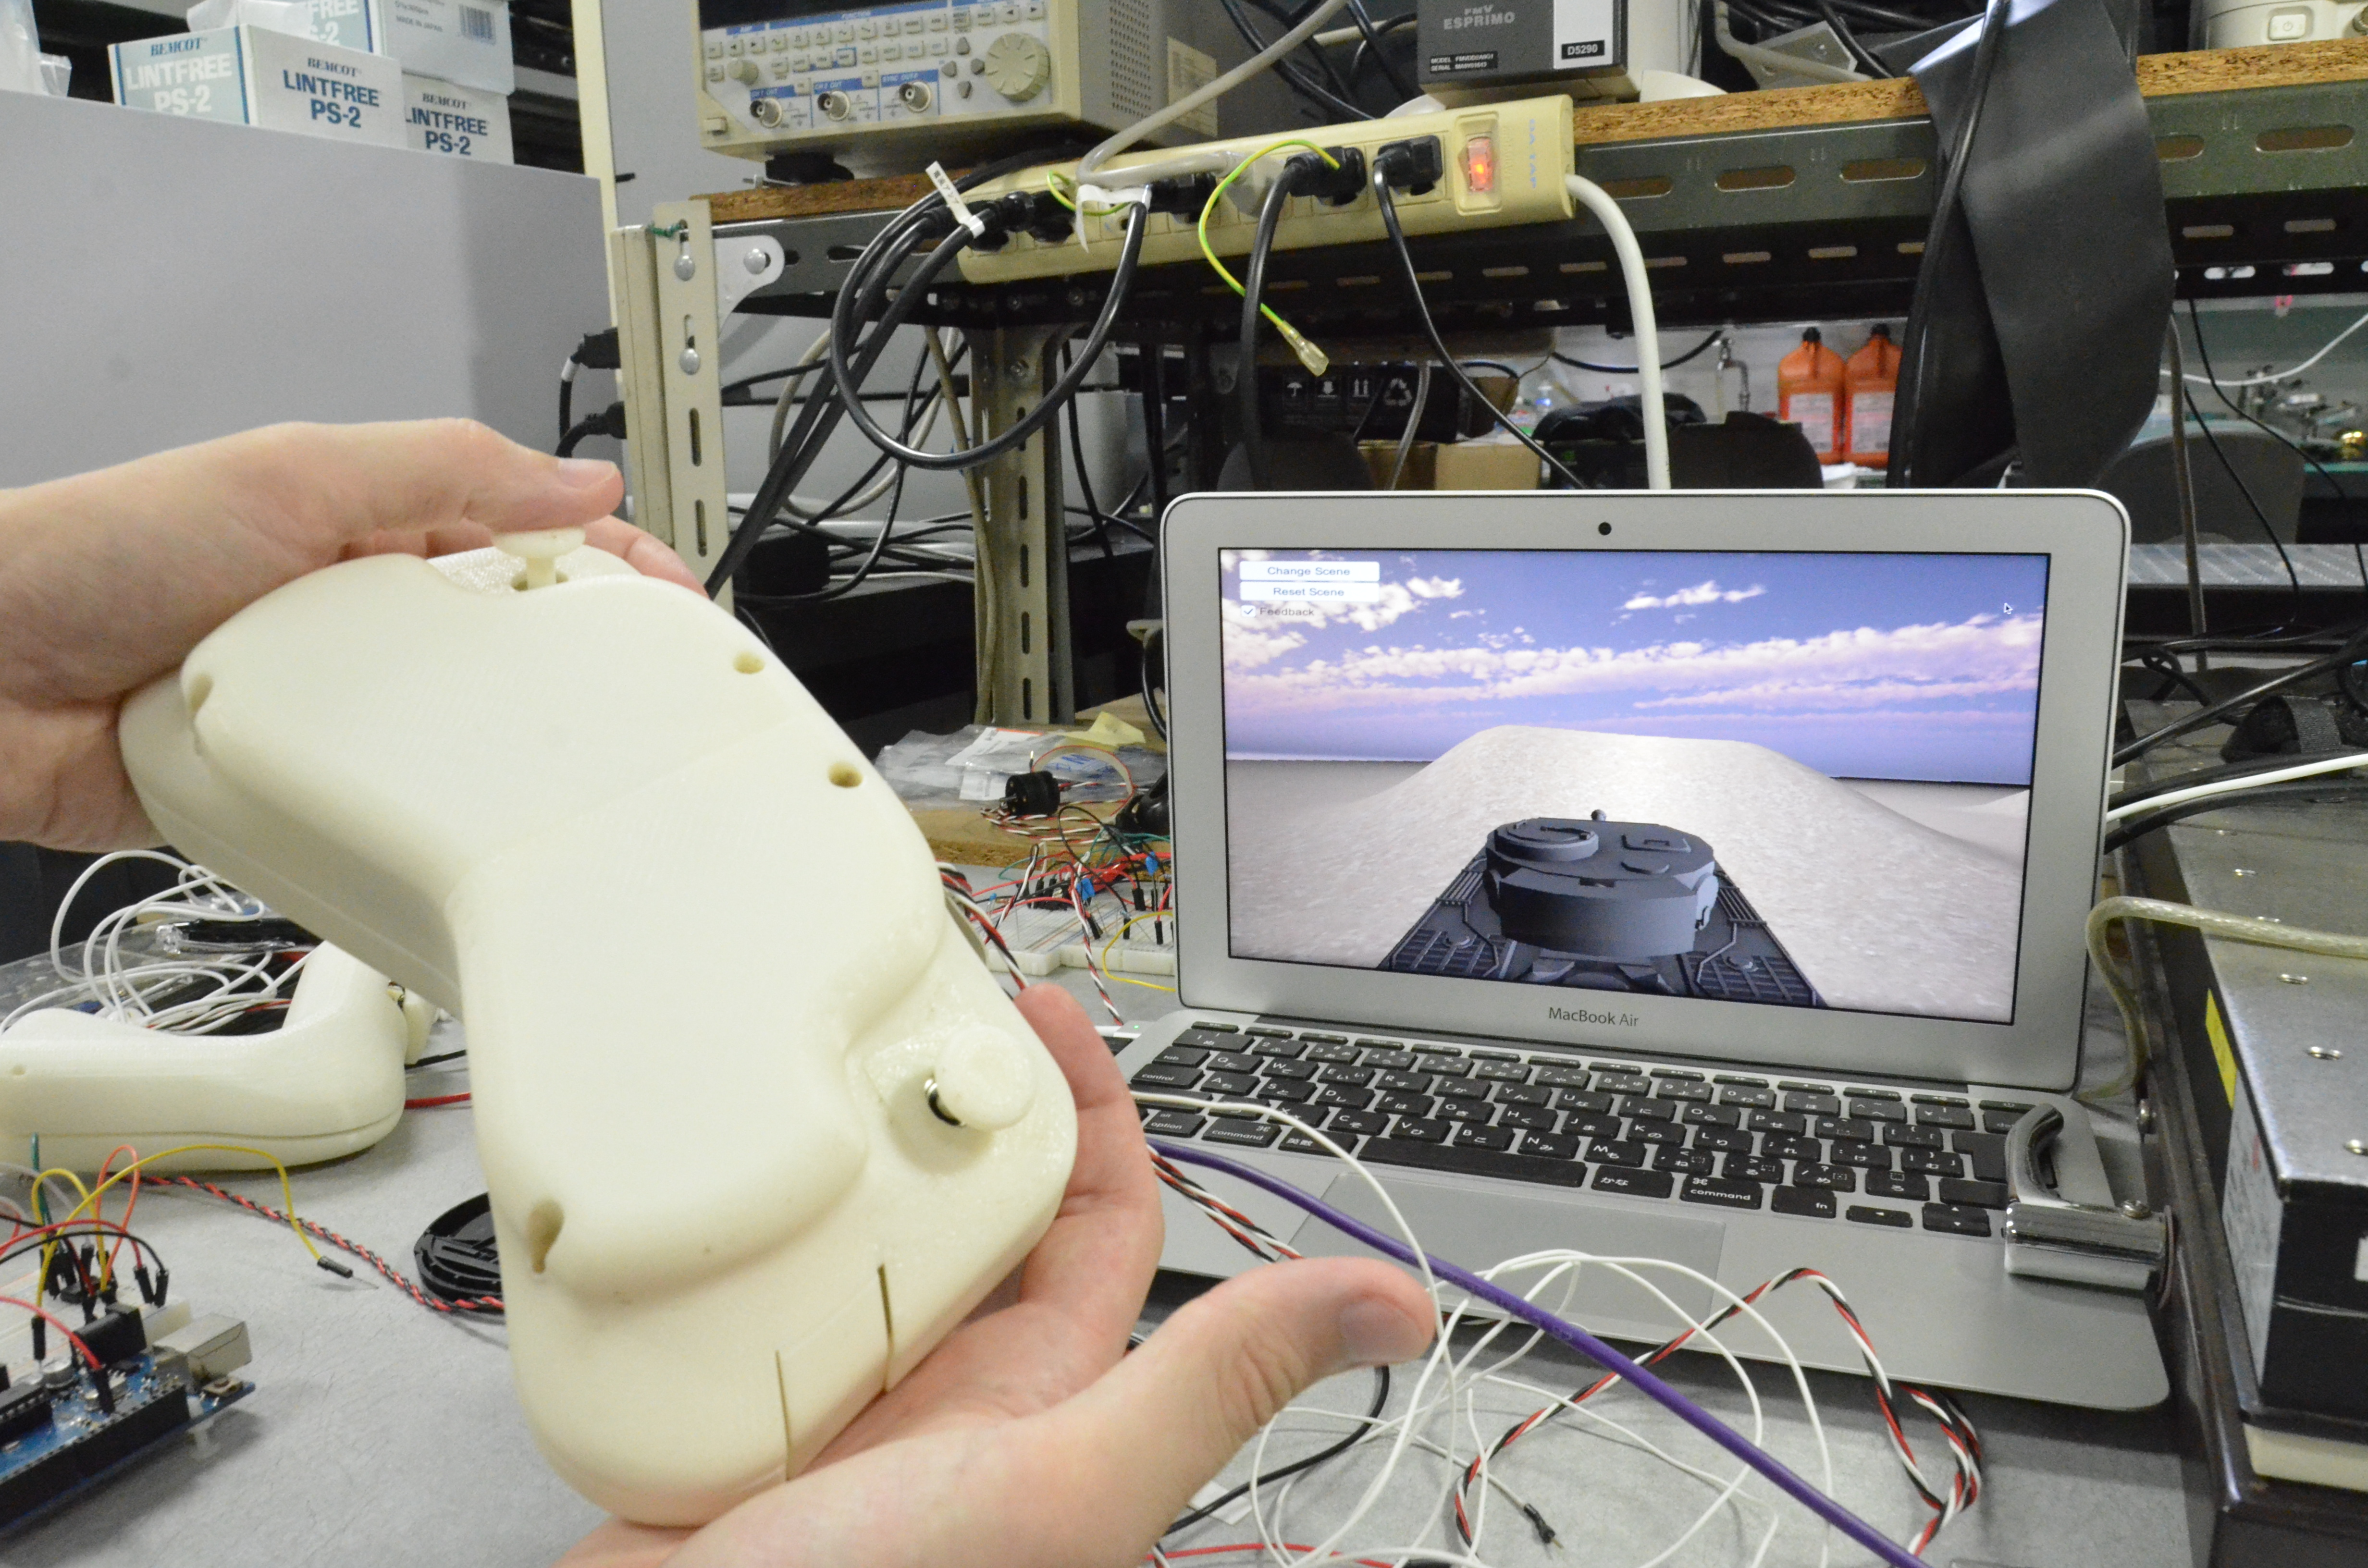
\includegraphics[width=0.6\linewidth]{Figs/unity_test_setup}
	\caption{Unity simulation test setup.}
	\label{fig:unity_test_setup}
\end{figure}
For testing the controller in the simulated world, the Unity program from the previous research of this project has been used. With minor modifications of the control software, the controller could be tested with different feedback for the two stimulators. This time, only the combined roll-pitch feedback law has been used.\\
Since all communication delays have been eliminated, the simulated tank reacted instantly to the user's command and its orientation angles is fed back. \\
There is no latency perceptible, neither when sending the commands, nor when receiving the feedback. The real-feel of the controller is better than before and even the maximum output force could be achieved when driving over the steep slopes of the environment. The range of the output force is appropriate for the desired feedback. And obstacles or slopes can be felt individually and intuitively on both sides.\\
This simulation-only test shows that the latency reported in the previous section does not stem from the implementation of the series elastic actuators and justifies the choice of this actuation system.\\

\subsubsection{Overall Evaluation of the PlayStation Controller}
Overall one can say that the controller has achieved the performance requirements stated in the beginning of the project. \\ \todo[inline]{maybe reference here}
The advantages of using SEA's are mostly the increased maximum output force and the decreased weight (VCM's tend to be very heavy due to the magnets). A drawback however is the size of the controller. The controller has been designed with several margins for dimensions and distances, leading to this bulky setup. If necessary, the design can be optimized in a future work, which would result in a much smaller controller than the current design.\\
Both control schemes (SEA and VCM) are straightforward and the output force can be controlled easily.\\
The disadvantages of the SEA implementation are the control speed and reaction time of the mechanical setup. As it has been shown in both testing environments, the mechanical response time is not the bottleneck in this setup.\\
Even though the maximum output force is enough to give a good feedback, it can be further increased. The motors that are used currently are not capable of compressing the springs to their maximal deflection. Therefore it is enough, to switch out the motors to have a higher torque. But when doing so, it should be verified, that the control speed of the motors do not affect the overall response time.\\
From the psychological points of view, the only shortcoming is the direction of the feedback which is application-specific. For this reason, and in order to write and test a parameter choice framework for future research projects, based on the current findings, a second controller has been designed.\\
        

\newpage